\documentclass[11 pt, a4paper]{article}

\usepackage{graphicx, amsmath,amssymb,amsfonts, dsfont, hyperref, framed, enumitem,color}
\usepackage[hmargin=2cm,vmargin=2cm]{geometry}
\usepackage{parskip} 
\usepackage{listings}
\renewcommand{\labelitemiii}{$\circ$}

\begin{document}
\begin{titlepage}
\begin{center}

\begin{figure}[h!]
\centering
\includegraphics[width=125mm]{Leeds_Logo.pdf}
\end{figure}

\vspace{4cm}
{\LARGE \textbf{MATH3001}: Project in Mathematics}\\

\vspace{1cm}
{\Huge \textbf{Flood Analysis}:Assessing and communicating mitigation of river floods to policy makers and the general public}\\
\vspace{5cm}
\textbf{Abbey Chapman}\\
ID: 201005685\\
\vfill
School of Mathematics\\
University of Leeds\\
2018/2019
\end{center}
\end{titlepage}

\tableofcontents 
\noindent \hrulefill

\newpage
\section{Introduction}
This project aims to use the analysis of flood data for multiple floods of a range of rivers as provided under the Freedom of Information Act by the Environment Agency and subsequently analyse the cost benefits of various proposed flood mitigation plans. \\
\textbf{Should I reference Toms' Github or the EA for Aire, Calder and Don data?}\\
Specifically we will explore:\\

\begin{framed}
\begin{itemize}
\item The possible flood mitigation plans that could be used.
\item The 2016 Boxing Day floods of the Rivers Aire, Calder and Don. This analysis will be done by the entire group.
\item The cost benefits of proposed flood mitigation plans to prevent any future floods along these rivers.
\item The 2012 November floods of the River Avon in both Warwick and Stratford-upon-Avon. This analysis will be done individually.
\item The cost benefits of proposed flood mitigation plans to prevent any future floods along the River Avon and specifically in these locales
\end{itemize}
\end{framed}
\textbf{How do I attach graphs, code, excel spreadsheets e.t.c.}\\
"It is estimated that flood damages in England have risen by around 60\% over the past 25 years and already exceed £1 billion per year in direct costs to communities and business".\cite{2}


\newpage
\section{The meaning of Flood Mitigation}
First of all, it should be made clear what Flood Mitigation actually is. To mitigate a flood is to reduce the amount of flooding, and thereby the damage as a result of such flooding, caused when a river breaks its banks.\\ 
This has been attempted since the very origins of non-nomadic humanity as the negative financial and social repercussions of a large flood (such as loss of property, crops, infrastructure and even life) are severe. Early examples of attempts to mitigate floods include the construction of stilt-houses by the Yue people in Ancient China around 7000 years ago.\cite{1}\\ 
In the modern world, we now have access to a vast array of possible flood mitigation schemes due to factors such as improvements in engineering and the implementation of a centralised  government with access to large sums of money with wich to implement flood mitigation schemes as well as the legal authority with which to do so.\\
In the course of this report, we will be investigating the effectiveness of such schemes at realistically reducing the volume of water discharged during a flood and thereby the cost effectiveness also, in the hopes that policy makers could make use of such analysis when implementing flood mitigation proposals.

\subsection{Possible methods of Flood Mitigation}
Examples of possible Flood Mitigation strategies include, but are not limited to:\\
\textbf{want to reference Onno here, can I?}
\begin{itemize}
\item High flood walls: increases the total volume of water a river can hold before it starts to flood.
\item River-bed widening: similar to high flood walls, it increases the capacity of the river itself.
\item Flood plain enhancement: increases the water retention of the ground itself within places at risk of flooding.
\item Natural Flood Management. This method includes examples such as:
\begin{itemize}
\item Tree planting:  improves the water retention of the ground as trees 'drink' water.
\item Peat restoration: improves the water retention of the ground.
\item Flow attenuation features: includes examples such as 'leaky dams' (like the ones that a beaver colony would build) that slow the flow of the river.
\end{itemize}
\item Sustainable Drainage Systems. This includes: \cite{3}
\begin{itemize}
\item Source Control:
\begin{itemize}
\item Green Roofs:
\item Rainwater Harvesting:
\item Water Butts:
\item Permeable Pavements:
\item Soakways:
\end{itemize}
\item Site Control:
\begin{itemize}
\item Filter Strips:
\item Trenches:
\item Swales:
\item Bioretention:
\item Geocellular/Modular Systems:
\end{itemize}
\item Regional Control:
\begin{itemize}
\item Infiltration Basins:
\item Detention Basins:
\item Ponds:
\item Wetlands:
\end{itemize}
\end{itemize}
\item The drawing down of drinking water reservoirs before predicted heavy rainfall:
\end{itemize}

\newpage
\section{Analysis of the 2016 Boxing Day floods along the River Aire}
\begin{figure}[h!]
\centering
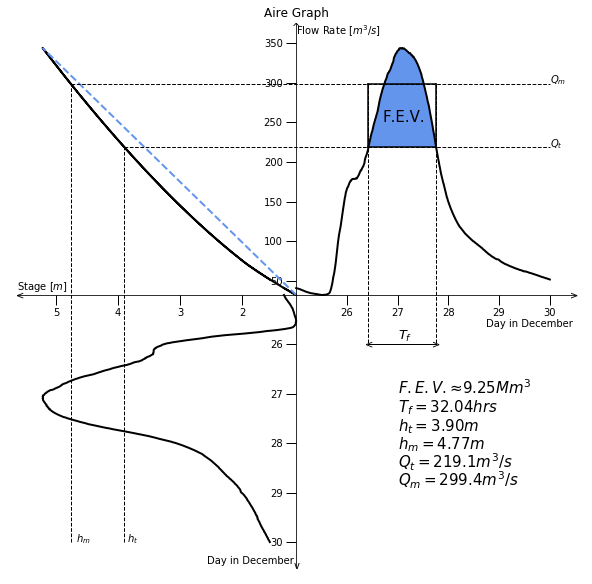
\includegraphics[width=125mm]{Aire-Quadrant_Graph.png}
\caption{Graph detailing the relationship between the Height and Flow Rate of the River Aire during the 2016 Boxing Day floods using data provided by the Environment Agency from the  monitoring station at Armley in Leeds.}
  \label{fig:Aire Graph}
\end{figure}

\ref{fig:Aire Graph}

\begin{thebibliography}{}
\bibitem{1} http://citeseerx.ist.psu.edu/viewdoc/summary?doi=10.1.1.383.1610
\bibitem{2} https://apps.warwickshire.gov.uk/api/documents/WCCC-1039-29
\bibitem{3} https://apps.warwickshire.gov.uk/api/documents/WCCC-1039-45
\end{thebibliography}

\newpage
\appendix
\section{Appendix}
{\bf The Aire Quadrant Graph - Python Code:}\\
{\em Should I include all data sets and code for each graph?}
\begin{lstlisting}
import matplotlib.pyplot as plt
import pandas as pd
import numpy as np

plt.rcParams["figure.figsize"] = [10,10]
plt.rcParams['axes.edgecolor']='white'
fig, ax = plt.subplots()

#Import the Data
armley=pd.read_csv('Aire Data.csv')
day = armley['Day in December']
flow = armley['Flow Rate (m^3/s)']
height = armley['Height (m)']

#Scale our Data
def scale(x):
    return ((x-min(x))/(max(x)-min(x)))
scaledday = scale(day)
scaledheight = scale(height)

#finding and using ht from the hm.
ht=3.9
HM = []
for i in height:
    if i>=ht:
        HM.append(i)
hm=sum(HM)/len(HM)

#Finding qt and qm.
def Q(x):
    if x<=0.685 and x>=0.165:
        y = (30.69*((x-0.156)**1.115))
    elif x<=1.917 and x>0.685:
        y = (27.884*((x-0.028)**1.462))
    elif x<=max(height) and x>1.917:
        y = (30.127*((x-0.153)**1.502))
    return(y)
qt = Q(ht)
qm = Q(hm)   

#Rating Curve
Flow = []
for i in height:
    if i<=0.685 and i>=0.165:
        Flow.append(30.69*((i-0.156)**1.115))
    elif i<=1.917 and i>0.685:
        Flow.append(27.884*((i-0.028)**1.462))
    elif i<=max(height) and i>1.917:
        Flow.append(30.127*((i-0.153)**1.502))

scaledFlow = []
for i in Flow:
    scaledFlow.append((i-min(Flow))/(max(Flow)-min(Flow)))


#Plot the Rating Curve using Q NOT the Flow Rate.
negheight = -scaledheight
ax.plot(negheight,scaledFlow,'black',linewidth=2)
ax.plot([0,-1],[0,1],'cornflowerblue',linestyle='--', marker='', linewidth=2)
#Originally the dotted line was wrong because it went to the positional origin
#and not the actual origin.

#Plot the Flow Rate and Height against the Date.
negday = -(scaledday)
ax.plot(scaledday, scaledFlow, 'black', linewidth=2)
ax.plot(negheight, negday, 'black', linewidth=2)

#Plot the lines illustrating ht,hm,qt,qm
#Scaling ht,hm,qt and qm.
scaledht = (ht-min(height))/(max(height)-min(height))
scaledhm = (hm-min(height))/(max(height)-min(height))
scaledqt = (qt-min(Flow))/(max(Flow)-min(Flow))
scaledqm = (qm-min(Flow))/(max(Flow)-min(Flow))
ax.plot([-scaledht,-scaledht],[-1,scaledqt], 'black', linestyle='--', linewidth=1)
ax.plot([-scaledhm,-scaledhm],[-1,scaledqm], 'black', linestyle='--', linewidth=1)
ax.plot([-scaledht,1],[scaledqt,scaledqt], 'black', linestyle='--', linewidth=1)
ax.plot([-scaledhm,1],[scaledqm,scaledqm], 'black', linestyle='--', linewidth=1)

#Fiddly plot to plot the box around the F.E.V. and the Tf line.
ax.plot([71/250,71/250,71/250],[scaledqt,scaledqm,-1/5], 'black', linestyle='--', linewidth=1)
ax.plot([69/125,69/125,69/125],[scaledqt,scaledqm,-1/5], 'black', linestyle='--', linewidth=1)
ax.plot([71/250,69/125],[-1/5,-1/5], 'black', linewidth=1)
ax.plot([71/250,71/250],[scaledqm,scaledqt], 'black',linewidth=1.5)
ax.plot([71/250,69/125],[scaledqm,scaledqm], 'black',linewidth=1.5)
ax.plot([71/250,69/125],[scaledqt,scaledqt], 'black',linewidth=1.5)
ax.plot([69/125,69/125],[scaledqm,scaledqt], 'black',linewidth=1.5)

#Formatting the ticks and the Axis.
ticks_x = [-3874/4091,-2874/4091,-1874/4091,-874/4091,1/5,2/5,3/5,4/5,1]
#This describes the position I want each tick to be on a graph with x axis
#from -1 to 1. Done by doing (2-min(height))/(max(height)-min(height))
#to find where 2 should be positioned on the axis.
ticks_y = [-1,-4/5,-3/5,-2/5,-1/5,3/52,17/78,59/156,7/13,109/156,67/78,53/52]
ax.set_xticks(ticks_x)
ax.set_yticks(ticks_y)
Ticks_x = [5,4,3,2,26,27,28,29,30]
Ticks_y = [30,29,28,27,26,50,100,150,200,250,300,350]
ax.set_xticklabels(Ticks_x)
ax.set_yticklabels(Ticks_y)
ax.spines['left'].set_position(('center'))
ax.spines['bottom'].set_position(('center'))
ax.spines['left'].set_color('black')
ax.spines['bottom'].set_color('black')
ax.tick_params(axis='x', colors='black', direction='out', length=10, width=1)
ax.tick_params(axis='y', colors='black', direction='out', length=10, width=1)

#Graph Title.
plt.title('Aire Graph')

#Graph labels.
plt.text(-4/6, -1,'$h_t$')
plt.text(-13/15, -1,'$h_m$')
plt.text(1, scaledqm,'$Q_m$')
plt.text(1, scaledqt,'$Q_t$')
plt.text(0.34,0.70,'F.E.V.', size=15)
plt.text(0.4,-0.18,'$T_f$',size=13)
plt.text(0.27,-0.213,'<')
plt.text(0.535,-0.213,'>')

#Axis Labels.
plt.text(0, 1.05,'Flow Rate $[m^3/s]$', size=10)
plt.text(0.75, -0.13,'Day in December', size=10)
plt.text(-0.35, -1.09,'Day in December', size=10)
plt.text(-1.1, 0.02,'Stage $[m]$', size=10)

#Arrows at end of Axis.
plt.text(-0.015,1.07,'^')
plt.text(-0.011,-1.11,'v')
plt.text(1.08,-0.013,'>')
plt.text(-1.105,-0.013,'<')

#Text on Graph.
plt.text(0.4,-0.4,'$F.E.V.≈9.25Mm^3$', size=15)
plt.text(0.4,-0.475,'$T_f=32.04hrs$', size=15)
plt.text(0.4,-0.55,'$h_t=3.90m$', size=15)
plt.text(0.4,-0.625,'$h_m=4.77m$', size=15)
plt.text(0.4,-0.7,'$Q_t=219.1m^3/s$', size=15)
plt.text(0.4,-0.775,'$Q_m=299.4m^3/s$', size=15)

#Fill in the F.E.V.
QT=[]
for i in scaledFlow:
    i = scaledqt
    QT.append(i)
#Because I have to make qt into a list otherwise I get an error because I'm
#comparing a list with a float.
a=np.array(scaledFlow)
b=np.array(QT)
#Puts lists into an array as opposed to a list. Means that Python finds it easier to
#compare the 2.
ax.fill_between(scaledday,a,b,where=a>=b,facecolor='cornflowerblue')

#Find the Tf
idx = np.argwhere(np.diff(np.sign(b - a))).flatten()
print(scaledday[idx])
def unscaleday(x):
    return (((max(day)-min(day))*x)+min(day))
c=unscaleday(0.283)
d=unscaleday(0.55)
Tf=(d-c)*24
print(Tf)
#find Tf in seconds
Tfs=Tf*(60**2)

#Find F.E.V
FEV=(qm-qt)*Tfs
print(FEV)
\end{lstlisting}
\end{document}